\providecommand{\main}{..}
\documentclass[main.tex]{subfiles}

\begin{comment}
\pgfdeclarelayer{nodelayer}
\pgfdeclarelayer{edgelayer}
\pgfdeclarelayer{connections}
\pgfsetlayers{edgelayer,nodelayer,connections,activity,lifelines,main}
\end{comment}

\begin{document}
\chapter{Software Design}

\section{System Design Overview}
\subsection{Microprocessor Platform}
The streaming capabilities and digital signal processing requirements of the system necessitated the choice of an appropriate microprocessor platform. 
A purely embedded solution was initially considered due to the availability of networking stacks such as FreeRTOS+UDP/IP and Light Weight IP (LWIP), the latter of which is available for ARM mbed platforms. 
This however would have limited audio and networking related software options that are available for general purpose operating systems such as Linux or QNX.

\medskip
As this was the first prototype for the project, the decision was made to select a Linux based platform as this would allow flexibility in the use of audio and streaming tools that are available for the OS. 
Benchmarking was conducted for potential platforms that would meet the system performance requirements as outlined in chapter 1, they are outlined in table \ref{table:HWPlatforms}.

\begin{table}[H]
    \centering  
    \caption{Benchmarking of Microprocessor Platform Specifications}
    \begin{tabu} to 0.8\textwidth { | l | l | l | l | l | l | }
        \hline
        \textbf{PLATFORM} &  \textbf{CPU} & \textbf{RAM} & \textbf{DAC} & \textbf{WLAN} & \textbf{PRICE}  \\
        \hhline{|=|=|=|=|=|=|}
        Raspberry Pi 3B\cite{rpiB} & ARM Cortex-A5 & 1GB & NO & YES & £34.00 \\
        & 1.4GHz quad-core & & & & \\
        \hline
        Hardkernel Odroid-CO\cite{odroid} & ARM Cortex-A5 & 1GB & NO & NO & £32.97 \\
        & 1.5GHz quad-core & & & & \\
        \hline
        iMX233-OLinuXino-MAXI\cite{olimex} & ARM 926EJ-S & 64MB & YES & NO & £42.13 \\
        & 454MHz single-core & & & & \\
        \hline
        Blueberry Pi\cite{blueberrypi} & ARM Cortex-A7 & 64MB & NO & YES & n/a \\
        & 1.2GHz single-core & & & & \\
        \hline
        Raspberry Pi Zero W\cite{rpi} & ARM 1176JZF-S & 512MB & NO & YES & £9.00 \\
        & 1.0GHz single-core & & & & \\
        \hline
        
        
    \end{tabu}
    
    \label{table:HWPlatforms}
    \end{table}

\medskip
%high performance boards (RPI3 & odroid)
%own board (blueberry pi & IMX6)

\medskip
With a single core Broadcom BCM2835 1GHz CPU, 500MB of RAM and no option to implement an eMMC over an SD card, the Raspberry Pi Zero W is significantly under-powered when compared to the other platforms. 
However, the much reduced cost of the device at approximately £9.00\cite{RpiPrice} is significantly less expensive than its counterparts. The very small size of the board, 65x30mm, was also desirable as it would take up much less space on the master PCB housed within the rear enclosure of the cabinet. 
The wiringPi library is also compatible with the Raspberry Pi Zero W (RPI) which would be convenient when interfacing with hardware peripherals such as the DAC, power-amplifier and user controls. The inclusion of a built in WLAN transceiver is particularly advantageous as this removes the need for a separate WLAN module/IC. 

\medskip
After careful consideration, this platform was selected due to the reasons outlined above. 
The chosen Linux distribution was Debian as it is the standard OS for the raspberry pi and allows easier configuration for real-time audio than other popular distributions such as Ubuntu. 
After the project was completed, an adapter board for the Odroid C0 was manufactured so it could replace the RPI in an attempt to gauge how the increased performance of the platform affected the performance of the overall system.
This testing did not come to fruition due to the project time-scale, however this is a potential area of future work. 

\subsection{Audio Streaming Platform}
Several streaming platforms and tools were benchmarked with regards to requirements as outlined in chapter 1. 
With many options under Linux, two potential approaches to implementing streaming were derived. 
A raw streaming protocol could be implemented at a low level or, a sound server with necessary streaming capabilities and a suitable C++ API could be used in order to distribute multiple streams to different speakers.

\medskip
%RTAUDIO & oRTP & raw-sockets

\medskip
%PulseAudio & JACK

\subsection{System Architecture}
The local and network audio streaming of the system is driven by Jack servers running on the user PC and each wireless speaker.
Using Jack allows for many popular audio programs that are Jack compatible, such as VLC media player, to integrate with the system with relative ease.
This also enables the fundamental use case of this project which is to allow any combination of audio streams to be routed to any combination of speakers.

\medskip
By running a Jack server with a ``net'' backend on each speaker (Netjack), the system capture port of each speaker is displayed as a standard Jack client with an input port. 
This is achieved by launching the server at boot for each speaker with the number of input ports set at one.
 
The user must use either the command line or a standard Jack front-end controller, such as QJackCtl for Linux or JackPilot for Mac, to launch the master Jack server. 
The Jack net manager must then be loaded by calling \lstinline{"jack_load netmanager"}  on the command line, this could however be easily automated using bash scripting.
Applications can then be connected to individual speakers using either the command line or front-end controller.
An example illustrating this can be seen in figure \ref{fig:jack-pilot} in which Jack pilot is used to connect left and right stereo outputs from VLC to separate speakers. 

\begin{figure}[H]
    \centering
    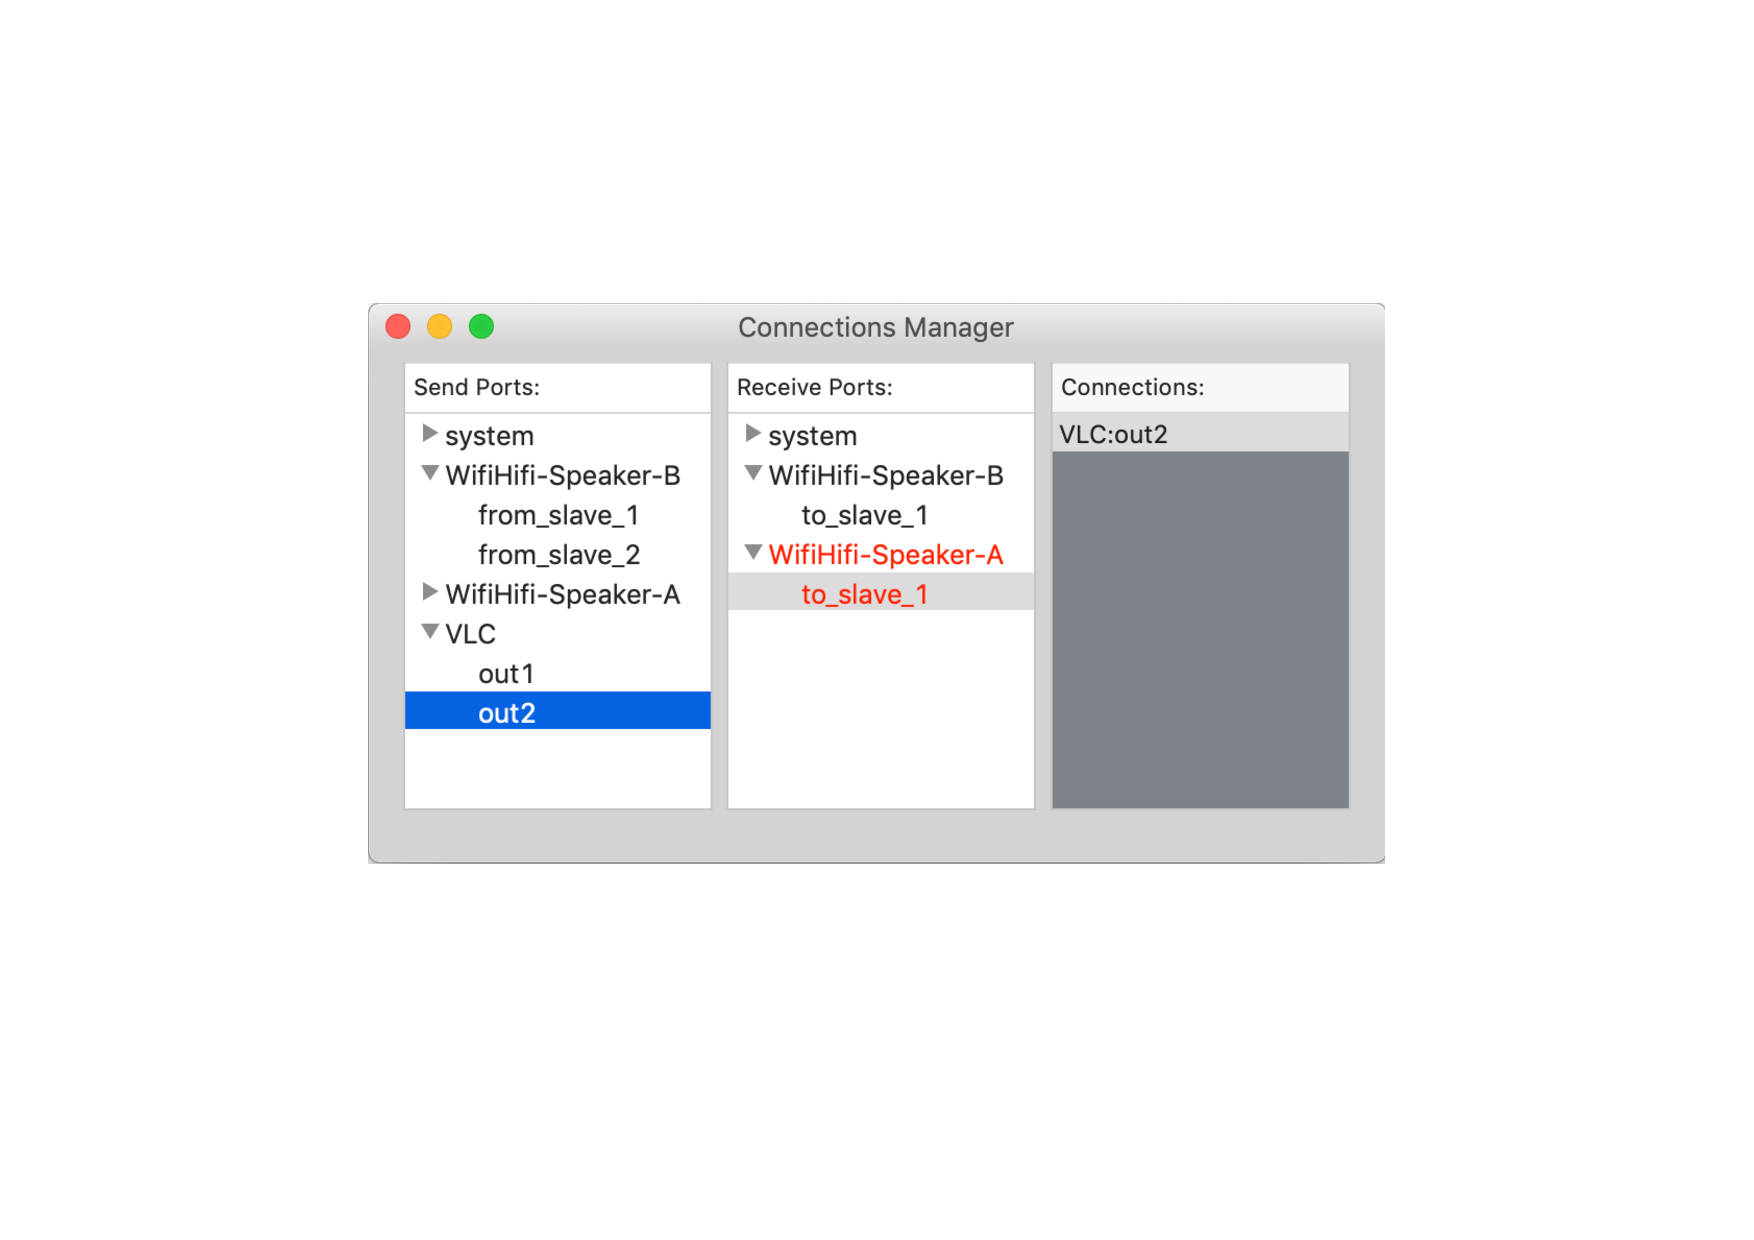
\includegraphics[scale=0.75]{./figs/jackpilot.pdf}        
    \caption{Using JackPilot to connect audio streams to speakers}
    \label{fig:jack-pilot}
\end{figure}

On the speaker side, the Jack server does not utilise a local sound card, this is because it is using the ``net'' backend which coordinates the audio stream transmitted from the Master server on the user device rather than using a local audio backend such as ALSA.
A custom Jack client therefore had to be written (WifiHifi Client) that would write to the sound-card directly using a local audio driver, in this project the Advanced Linux Sound Architecture (ALSA) was used to achieve this.
The client's additional purposes are to perform necessary signal processing, synchronise the output stream to the Jack server, and listen for incoming datagrams from the user desktop app (WifiHifi Controller).
This can be demonstrated in figure \ref{fig:JACKclients}, a high-level system diagram.

\begin{figure}[H]
    \centering
    \begin{tikzpicture}
        \begin{umlpackage}{Speaker A}
            \umlsimpleclass{ALSA/I2S Interface A}
            \umlsimpleclass[x=0, y=-1.5]{WifiHifi Client A}
            \umlsimpleclass[x=0, y=-3]{Netjack Server A}

            \umluniassoc{WifiHifi Client A}{ALSA/I2S Interface A}
            \umluniassoc{Netjack Server A}{WifiHifi Client A}        
        \end{umlpackage}
        
        \begin{umlpackage}[x=7, y=0]{Speaker B}
            \umlsimpleclass{ALSA/I2S Interface B}
            \umlsimpleclass[x=0, y=-1.5]{WifiHifi Client B}
            \umlsimpleclass[x=0, y=-3]{Netjack Server B}
    
            \umluniassoc{WifiHifi Client B}{ALSA/I2S Interface B}
            \umluniassoc{Netjack Server B}{WifiHifi Client B}        
        \end{umlpackage}

        \begin{umlpackage}[x=2, y=-7]{User Device}
            \umlsimpleclass[x=1.5]{Master JACK Server}
            \umlsimpleclass[x=0, y=-1.5]{Client App 1}
            \umlsimpleclass[x=4, y=-1.5]{Client App 2}

            \umluniassoc{Client App 1}{Master JACK Server}    
            \umluniassoc{Client App 2}{Master JACK Server}        
        \end{umlpackage}

        \umldep[geometry=|-|, name=dep]{User Device}{Speaker A}
        \umldep[geometry=|-|]{User Device}{Speaker B}
        \umlnote[x=9.5, y=-5]{dep-1}{UDP Network Transport}

    \end{tikzpicture}
    \caption{High-level JACK-based system diagram}
    \label{fig:JACKclients}
\end{figure}

\pagebreak
\section{WifiHifi Client}
\subsection{Overview}
%threads, class hierarchy etc
The client was written using the QtJack library, a C++ wrapper for the JACK C API that allows integration with the Qt multitasking environment.
On startup, a JACK server with the ``net'' backend is launched before the client is activated\footnote{registered by the server}, the client is created and connected to the server.
The top level classes (instantiated in \lstinline{main()}) are then created and referenced to the appropriate classes before all threads and the Qt executive are started.

\medskip
The system runs two main threads, the receiver thread that simply receives audio from the the server before writing it to a ring-buffer, and a dedicated processing thread that performs necessary DSP and outputs the audio to hardware.
A separate thread is used for processing such that the processing can continue to run without being interrupted by the server, a drift correction algorithm, discussed in more detail later, and a wait condition, in the processing thread, are used to ensure that both streams remain aligned.
A UML class diagram can be seen in figure \ref{fig:client-uml}.
\def \xval {5}
\def \yval {-6}
\def \scaleuml {0.75}
\begin{figure}[H]
    \centering
    \begin{tikzpicture}[scale=0.4, every node/.style={scale=1}]
        \begin{umlpackage}[fill=creamy]{WifiHifi Client}
            %declare classes/packages
            \umlclass[x=0, y=\yval, scale=\scaleuml, type=class]{AlsaController}{}
            {
                WriteInterleaved() \\
                FramesReady() \\
                Rewind()
            }
            \umlsimpleclass[x=0,y=0, scale=\scaleuml, fill=blue!20, type=library]{asoundlib}
            \umlclass[x=2.5*\xval,y=0.2\yval, scale=\scaleuml, type=class]{HardwareController}{}
            {
                SetVolume() \\
                PowerDownISR() \\
                VolumeISR()
            }
            \umlsimpleclass[x=2.5*\xval,y=0, scale=\scaleuml, type=library, fill=blue!20]{wiringPi}
            \umlclass[x=5*\xval,y=\yval,fill=green!20, scale=\scaleuml, type=class]{SlaveProcessor}
            {
                ringBuffer : boost::ringBuffer
            }
            {
                process() \\
                bufferSize() \\
                sampleRate() \\
                bitDepth()
            }
            \umlsimpleclass[x=5*\xval,y=0,fill=green!20, scale=\scaleuml, type=class]{QtJack::Processor}
            \umlsimpleclass[x=7*\xval,y=0.4*\yval,fill=green!20, scale=\scaleuml, type=class]{QtJack::Server}
            \umlclass[x=5*\xval,y=2.5*\yval, scale=\scaleuml, type=class]{boost::circularbuffer}
            {}
            {
                front() \\
                pop\textunderscore front() \\
                push\textunderscore back()
            }
            \umlsimpleclass[x=0,y=4*\yval, scale=\scaleuml, type=class]{IIRFilter}
            \umlsimpleclass[x=1.5*\xval,y=4*\yval, scale=\scaleuml, type=class]{FIRFilter}
            \umlsimpleclass[x=3*\xval,y=4*\yval, scale=\scaleuml, type=class]{Fir1}
            \umlclass[x=2.5*\xval,y=2.5*\yval, fill=red!20, scale=\scaleuml, type=class]{AlsaWorker}{}
            {
                Work() \\
                EQSettings() \\
                AdjustMid() \\
                AdjustTreble() \\
                AdjustBass() \\
                EnableEQ() \\
                DisableEQ() 
            }

            \umlclass[x=0,y=2.5*\yval, fill=orange!30, scale=\scaleuml, type=class]{ClientController}{}
            {
                readyRead()
            }

            %connections
            \umlaggreg{AlsaController}{AlsaWorker}
            \umlaggreg{HardwareController}{AlsaWorker}
            \umlcompo{IIRFilter}{AlsaWorker}
            \umlcompo{FIRFilter}{AlsaWorker}
            \umlaggreg{SlaveProcessor}{AlsaWorker}
            \umlaggreg{boost::circularbuffer}{AlsaWorker}
            \umlcompo{boost::circularbuffer}{SlaveProcessor}
            \umlaggreg[geometry=-|]{SlaveProcessor}{QtJack::Server}
            \umlinherit{SlaveProcessor}{QtJack::Processor}
            \umlcompo{Fir1}{FIRFilter}
            \umldep{AlsaController}{asoundlib}
            \umldep{HardwareController}{wiringPi} 
            \umlaggreg{ClientController}{AlsaWorker}

        \end{umlpackage}
    \end{tikzpicture}
    \caption{UML Collaboration/Class Diagram of WifiHifi JACK Client}
    \label{fig:client-uml}
\end{figure}

\subsection{JACK Interface}
To interface the client software with JACK, the \lstinline{SlaveProcessor} class was written that contains an asyncronous callback \lstinline{process()} that is used by the server to notify when a buffer of samples has been delivered to the client's input ports.
When called, the \lstinline{SlaveProcessor} reads this from the input port's buffer and immediately writes all samples to the tail of a ring-buffer.
One of the GPIO pins is also toggled, this is used for debugging to determine if a callback has been missed.
Callbacks should be called by the server at a rate determined by the following equation where $N$ and $f_{s}$ represent the buffer size and sample rate respectively.
\begin{equation}
T_{callback} = \frac{N}{f_{s}}
\end{equation}   

Both the sample rate and buffer size are determined by the server configuration on the master device (user's PC), it is recommended that these be set to 44.1kHz and $\geq$4096 for sampling rate and buffer size respectively for normal operation.
The \lstinline{SlaveProcessor} takes a reference to the Client in its constructor, it can therefore determine both the sample rate and buffer size allowing other classes in the client to query this information through the \lstinline{SlaveProcessor} by calling its relevant public methods.

\begin{figure}[H]
    \centering
    \begin{tikzpicture}
        \umlclass[scale=0.75]{WifiHifi::AlsaWorker}
        {  
        + boost::circular\textunderscore buffer : ringBuffer \\
        - QtJack::AudioPort : in \\
        - Qmutex : mutex
        }
        {
        SlaveProcessor(QtJack::Client\&) \\
        \char`\~ SlaveProcessor() \\
        + EQSettings() : threeBand\textunderscore t \\
        + process(int) : void \\ 
        + bufferSize() : int \\
        + sampleRate() : int \\
        + bitDepth() : int 
        }

    \end{tikzpicture}
    \caption{SlaveProcessor UML Class Diagram}
    \label{fig:alsa-uml}
\end{figure}

\subsection{ALSA Interface}
The client utilises the ALSA API as a means to write the audio stream to hardware.
Since the 1st generation PCB utilised the PCM5102A ,the same DAC from the phatDAC audio evaluation board, the device's audio was reconfigured from its default audio interface to the I2S interface using the phatDAC's device tree\cite{phatDAC-tree}.
This device tree simply reconfigures for I2S output over the relevant RPI pins, this meant that it could be used with the 2nd generation board as well.

\medskip
ALSA configuration/setup and the write method are contained within the \lstinline{AlsaController} class, this aims to abstract the ALSA API from other classes.
On construction, setup configuration is performed by setting relevant parameters such as the sample rate, buffer size and buffer access type.
The \lstinline{WriteInterleaved()} method is used to write an interleaved buffer of samples to the DAC, if the initial write fails (i.e. an over-run or under-run occurs) then an attempt is made to recover by resetting the device using the \lstinline{RecoverXRuns} method.
The class also contains methods to rewind the stream (\lstinline{Rewind()}) and query the number of samples available for ALSA to write for the current cycle(\lstinline{FramesReady()}).

\medskip
The class \lstinline{AlsaWorker()} is run in a dedicated thread and performs the intensive signal processing, synchronises the outbound and inbound audio streams, and writes to the output.
It's main routine, \lstinline{Work()}, is synchronised to the receiver thread using a wait condition that blocks the thread until the receiver has notified that it has completed writing all samples to the ring-buffer.
This ensures that no buffer xruns occur due to the processing thread (ALSA) running ahead of the receiver (JACK). A UML class diagram of the ALSA related classes can be seen in figure \ref{fig:alsa-uml}.

\begin{figure}[H]
    \centering
    \begin{tikzpicture}
        \umlclass[scale=0.75]{WifiHifi::AlsaWorker}
        {  
        - FIRFilter* : firWoof \\
        - FIRFilter* : firTweet \\
        - IIRFilter* : midEq \\
        - IIRFilter* : bassEq \\
        - IIRFilter* : trebleEq \\
        - IIRFilter* : notchCorrection \\
        - IIRFilter* : zobelCorrection \\
        - AlsaController* : dac \\
        - int64\textunderscore t* : alsaBuffer \\
        - SlaveProcessor* : processor \\
        - double* : integDeltaK \\
        - double* : resampleMean \\
        - double* : smoothBuffer \\
        - float : atten \\
        - bool : eqEnabled
        }
        {
        AlsaWorker(QtJack::Client\&, SlaveProcessor*) \\
        \char`\~ FIRFilter() \\
        + EQSettings() : threeBand\textunderscore t \\
        + AdjustMid(filterConfig\textunderscore t) : double \\ 
        + AdjustBass(filterConfig\textunderscore t) : void \\
        + AdjustTreble(filterConfig\textunderscore t) : void \\
        + EnableEQ() : void \\
        + Attenuate() : void\\
        + Work() \\
        - DriftCorrection() : int \\
        - HighpassCoeffs(int, double) : bool \\
        - AllpassCoeffs(int) : bool
        }

        \umlclass[x=7.5, y=0, scale=0.75]{WifiHifi::AlsaController}
        { 
        - snd\textunderscore pcm\textunderscore hw\textunderscore params\textunderscore t* : hwParams \\
        - snd\textunderscore pcm\textunderscore t* : playbackHandle \\
        - unsigned int : periodSize  \\
        - unsigned int : sampleRate     
        }{
        AlsaController(QtJack::Client\&, const char*) \\
        \char`\~ AlsaController() \\
        + WriteInterleaved(double) : double \\ 
        + FramesReady() : uint32\textunderscore t \\
        + Rewind(uint32\textunderscore t) : bool \\
        - RecoverXRuns(int)) : bool 

        }

        \umlunicompo[geometry=-|]{WifiHifi::AlsaController}{WifiHifi::AlsaWorker}
    \end{tikzpicture}
    \caption{FIRFilter UML Class Diagram}
    \label{fig:alsa-uml}
\end{figure}

\medskip
Two copies of each sample are processed separately before being interleaved and written, these are interleaved in a single output buffer.
By default, the Netjack interface encodes all samples as 32-bit floating point, the output buffer is therefore allocated as a 64-bit array the size of which is determined by the buffer size configuration of the master JACK server.
The least significant 32 bits contain the sample to be sent to the woofer, the most significant 32 bits are the sample to be sent to the tweeter. 
The PCM5102A does not support floating point audio, the samples are therefore scaled to 32-bit, arranged into a single sample, and placed into the buffer. 
This buffer is then referenced to the \lstinline{AlsaController::WriteInterleaved()} method, outputting the samples over the I2S interface.
This can be seen in the following listing.

\begin{lstlisting}[language=c++, caption={Interleaving Tweeter/Woofer Stream}]
        leftSample32 = static_cast<int64_t>(leftSample*0x10000000);
        leftSample32 = leftSample32 & 0x00000000FFFFFFFF;
        rightSample32 = static_cast<int64_t>(rightSample*0x10000000);
        rightSample32 = rightSample32 << 32;
        rightSample32 = rightSample32 & 0xFFFFFFFF00000000; 
        currentSample = rightSample32 | leftSample32;                           
        m_alsaBuffer[pos] = currentSample;
    }
    if ( !m_dac->WriteInterleaved(m_alsaBuffer, newBuffSize) )
    {
        /* fatal, can't recover from xruns */
        cout << "ALSA WORKER: failed to write to device" << endl;
        exit(1);
    }
\end{lstlisting}



\section{Signal Processing}
In order to reduce electronic component count, DSP has been used to implement signal processing tasks that would typically be achieved using analogue circuitry.
These include the crossover filters, frequency correction circuitry and tone controls.
\subsection{Crossover Filters}
A two-way crossover circuit is typically used to split the high and low frequencies between the tweeter and woofer respectively around a common crossover frequency using highpass and lowpass filters;
the specific value of this crossover frequency is chosen based on the frequency response of each driver.
As can be seen in figure \ref{fig:tweeter-response}, the resonant frequencies of the tweeter is approximately 1.5kHz.
The crossover frequency was initially set at 3kHz, an octave above the tweeter's resonant frequency.
After some trial and error, it was decided that a crossover frequency of 2.5kHz resulted in the most pleasant response, this is obviously subjective however implementing the filters in software allows them to be varied easily.

\begin{figure}[H]
    \centering
    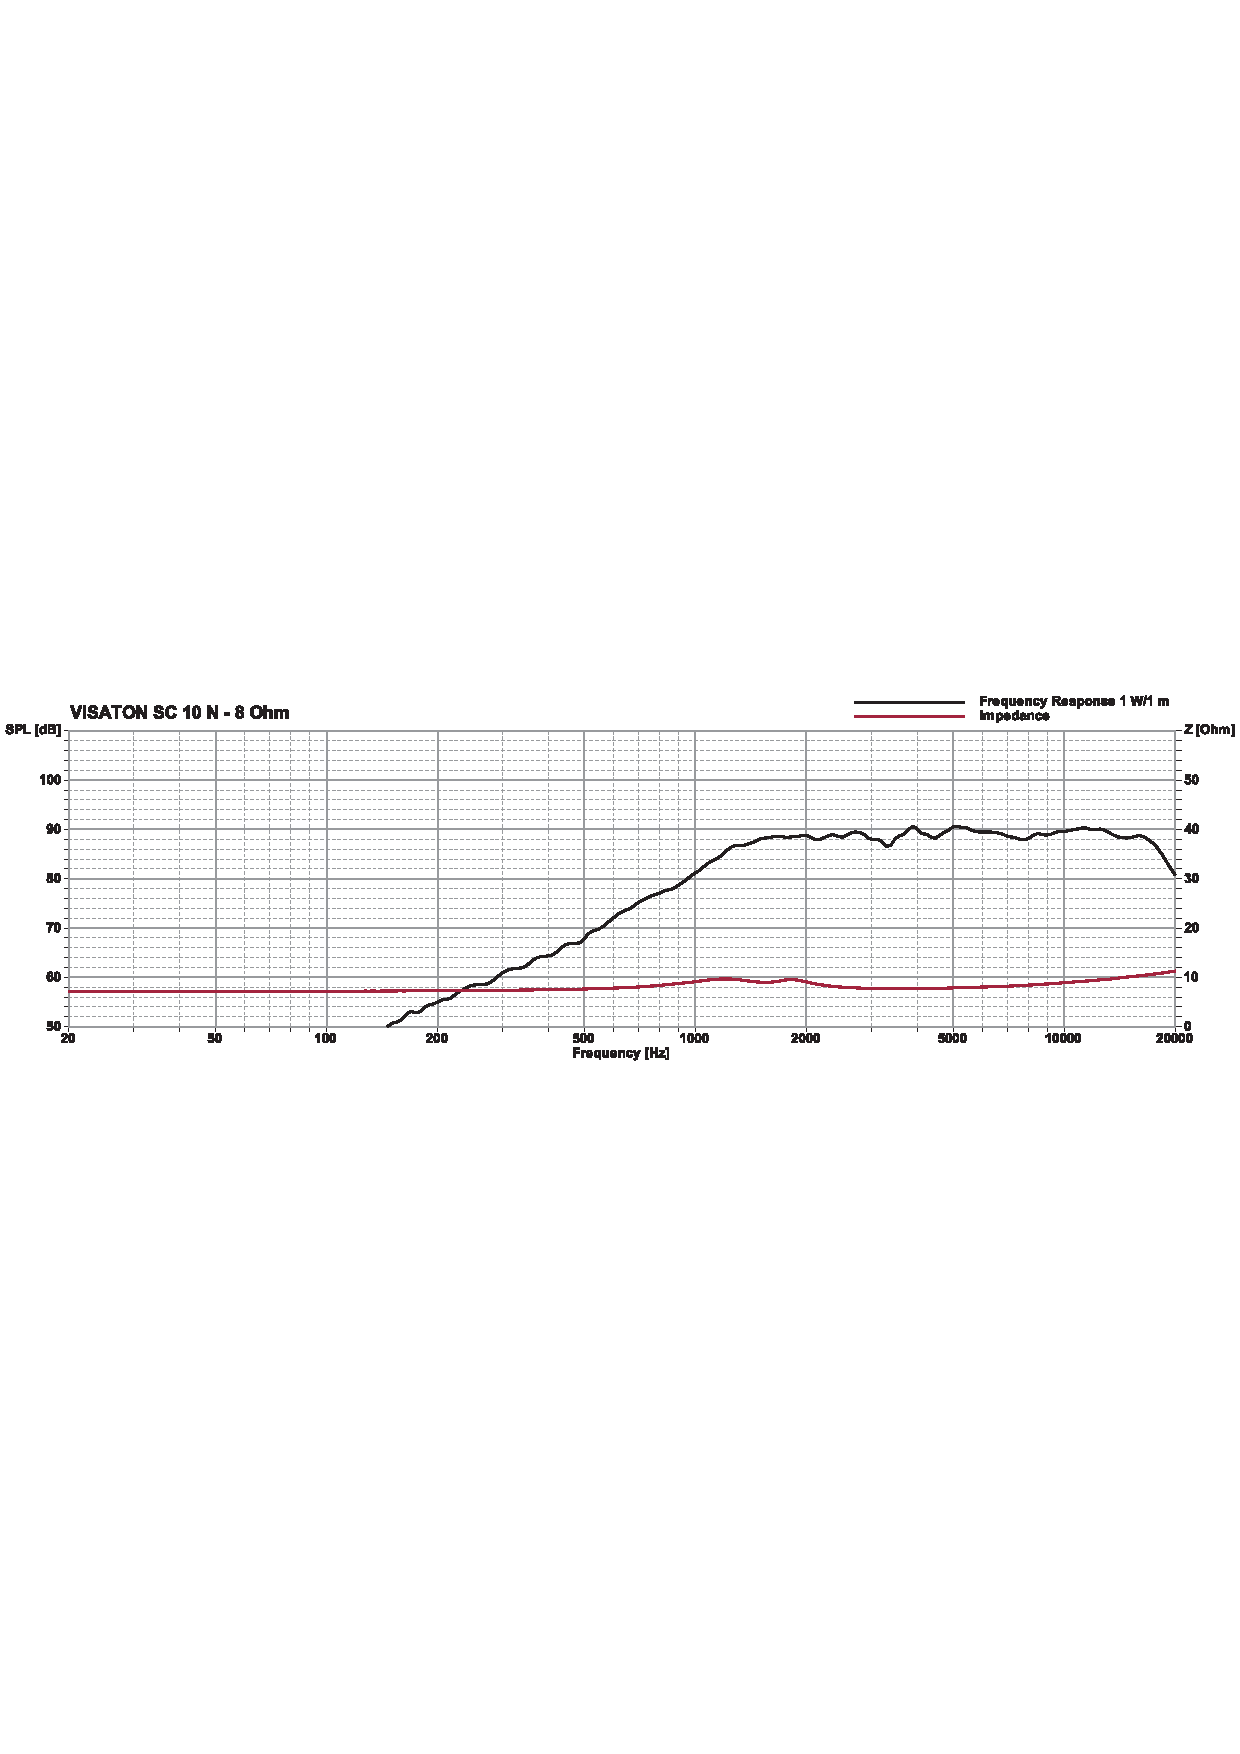
\includegraphics[scale=0.6]{./figs/tweeter-response.pdf}        
    \caption{Impedance and Amplitude response of Tweeter with respect to Frequency\cite{tweeter}}
    \label{fig:tweeter-response}
\end{figure}

\begin{figure}[H]
    \centering
    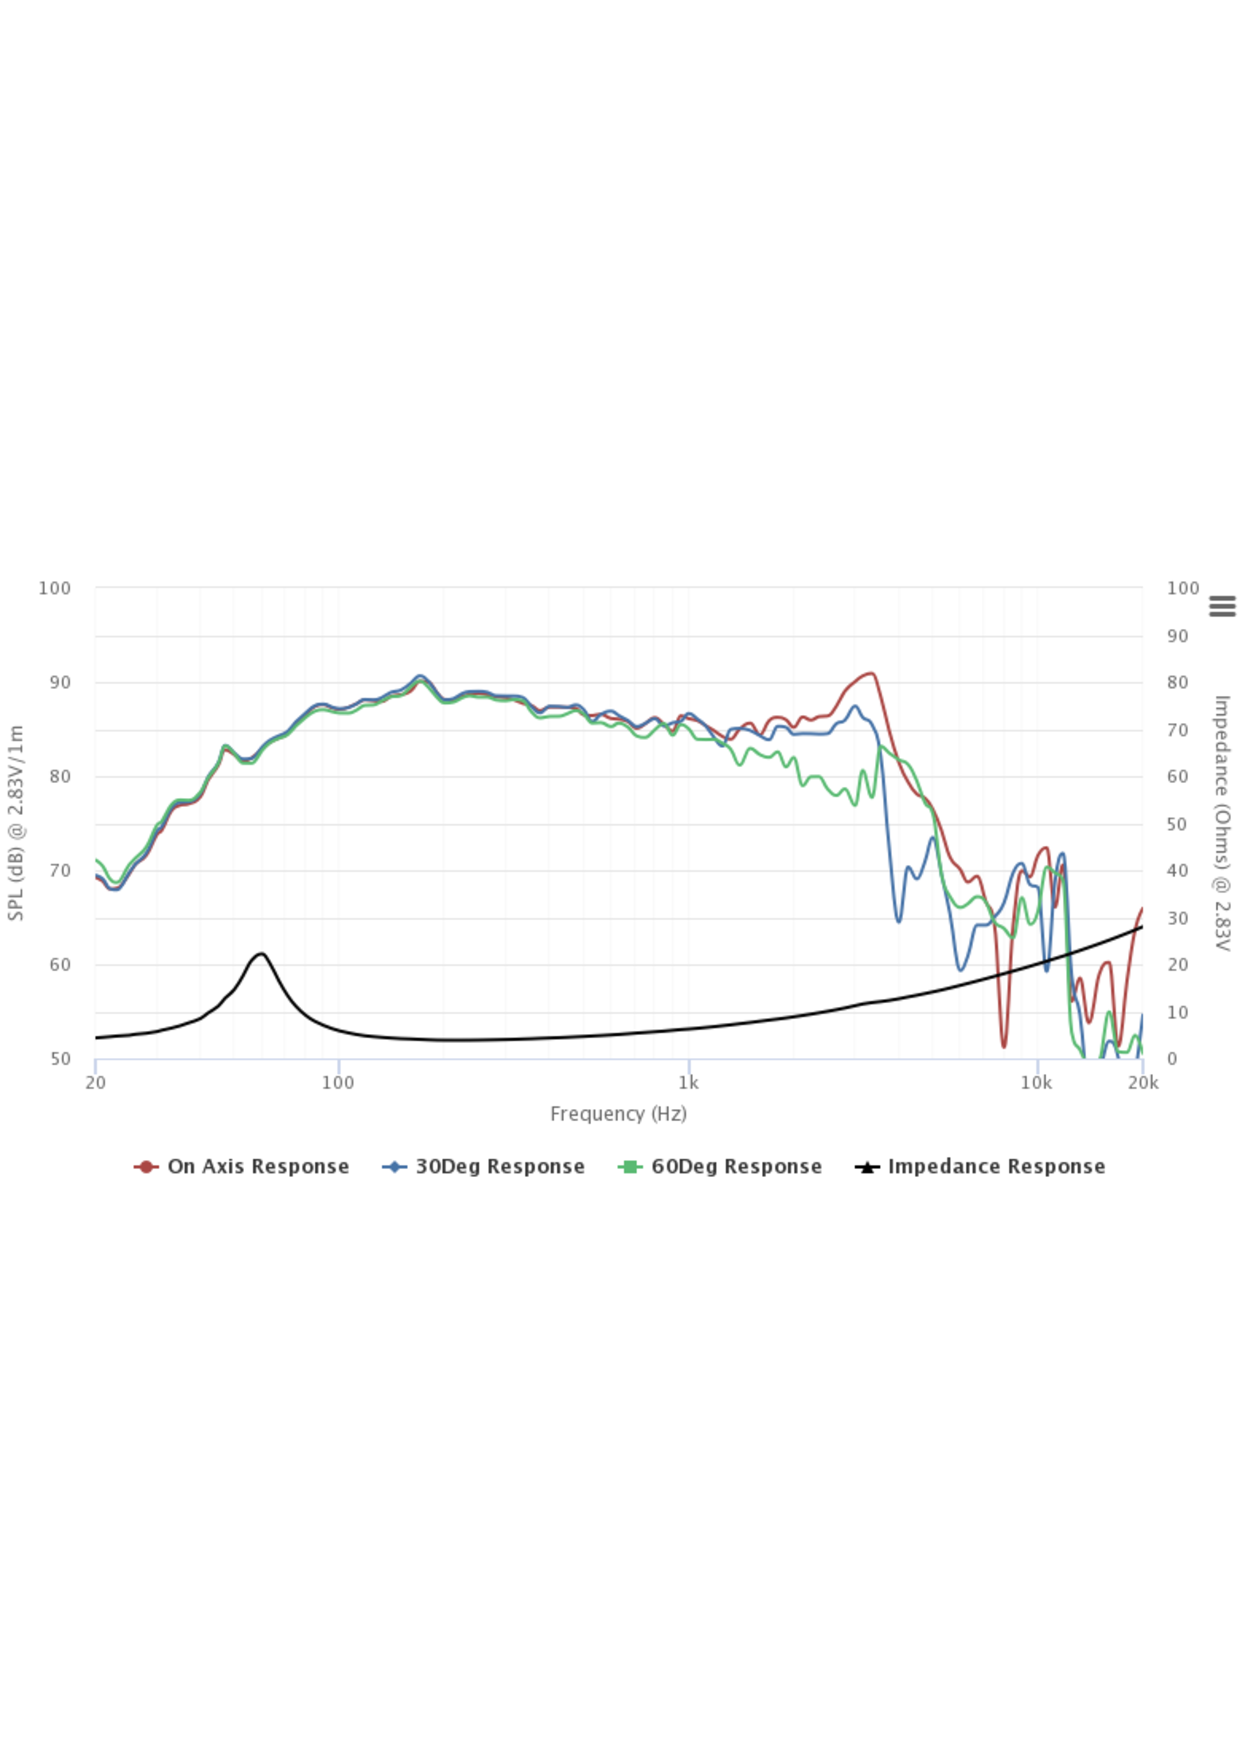
\includegraphics[scale=0.5]{./figs/woofer-response.pdf}        
    \caption{Impedance and Amplitude response of Woofer with respect to Frequency\cite{woofer}}
    \label{fig:woofer-response}
\end{figure}

Each crossover filter was implemented using an FIR filter with 75 coefficients. 
A class (\lstinline{FIRFilter}) was written that calculates the coefficients and performs sample by sample filtering of an input audio sample. 
The filter implementation utilises a real-time FIR filter library written by Bernd Porr\cite{fir1} (\lstinline{fir1}), the calculated coefficients are referenced by an instantiated \lstinline{fir1} object that performs the convolution algorithm. 
A UML class diagram of the \lstinline{FIRFilter} class can be seen in figure \ref{fig:fir-uml}.

%\begin{comment}
\begin{figure}[H]
    \centering
    \begin{tikzpicture}
        \umlclass{WifiHifi::FIRFilter}{  
        - Fir1* : fir \\
        - double* : coeffs 
        }{
        <<constructor>> FIRFilter() \\
        <<destructor>> \char`\~ FIRFilter() \\
        + filter(double) : double \\ 
        + reset() : void \\
        - LowpassCoeffs(int, double) : bool \\
        - HighpassCoeffs(int, double) : bool \\
        - AllpassCoeffs(int) : bool
        }

        \umlclass[x=7.5, y=0]{Fir1}{ 
        - unsigned : taps \\
        - double* : buffer \\
        - double* : coefficients 
        }{
        <<constructor>> Fir1() \\
        <<destructor>> \char`\~ Fir1() \\
        + filter(double) : double \\ 
        + reset() : void \\
        + zeroCoeff() : void \\
        }

        \umlunicompo[geometry=-|]{Fir1}{WifiHifi::FIRFilter}
    \end{tikzpicture}
    \caption{FIRFilter UML Class Diagram}
    \label{fig:fir-uml}
\end{figure}
%\end{comment}

\medskip
On object construction, the class will numerically calculate the filter impulse response for the specified filter type and number of coefficents/taps. 
The impulse responses are calculated using the following equations\cite{DSP-berndporr}, where $h(n)$, $n$ and $\omega _c$ represent the filter impulse response, current sample and angular cutoff frequency ($\omega _c = 2\pi f_c$) respectively.

\begin{equation}
    h_{lowpass}(n) =
    \begin{cases}
        \frac{\omega _c}{\pi}     &\text{for \(n=0\)}  \\
        \frac{1}{\pi n}sin(\omega _cn)    &\text{else}
    \end{cases}
\end{equation}
\begin{equation}
    h_{highpass}(n) =
    \begin{cases}
        1-\frac{\omega _c}{\pi}     &\text{for \(n=0\)}  \\
        -\frac{1}{\pi n}sin(\omega _cn)    &\text{else}
    \end{cases}
\end{equation}

\medskip
The impulse response is then windowed with a Blackman window.
This was chosen due to its greater attenuation in the stop band than a Hamming window\cite{DSP-berndporr}.
It was calculated using the following equation where $w(n)$, $n$ and $M$ are the window function, current sample and number of coefficients/taps respectively.

\begin{equation}
    w(n)=
    0.42 + 0.5cos\left(\frac{2\pi n}{M}\right) + 0.08cos\left(\frac{4\pi n}{M}\right)
\end{equation}

Figures \ref{fig:highpass-fft} and \ref{fig:lowpass-fft} show plots of FFTs recorded for the highpass and lowpass filters respectively.
They were obtained by probing the relevant DAC output with a digital oscilloscope line, passing Gaussian white noise through the WifiHifi client and exporting the data to a csv file;
all other software filtering was disabled.

\def \minfft{0}
\def \maxfft{15000}

\begin{figure}[H]
    \begin{tikzpicture}
        \begin{axis}[
            width=\textwidth, 
            height=\axisdefaultheight,
            xlabel={Frequency},
            ylabel={Gain(dB)},
            xmin=\minfft,
            xmax=\maxfft, 
            %xmode=log,     
        ]
        %\addplot table [mark=none, x=t, y=a, col sep=comma] {./data/saleae-outputs/sync.csv};
        
        \addplot table [mark=none, x=f, y=a, col sep=comma] {./data/csvs/test_001_10.csv};
        \end{axis}
    \end{tikzpicture}
    \caption{Raw FFT of Highpass Crossover Filter from Scope}
    \label{fig:highpass-fft}
\end{figure}

\begin{figure}[H]
    \begin{tikzpicture}
        \begin{axis}[
            width=\textwidth, 
            height=\axisdefaultheight,  
            xlabel={Frequency},
            ylabel={Gain(dB)},  
            xmin=\minfft,
            xmax=\maxfft,     
        ]
        %\addplot table [mark=none, x=t, y=a, col sep=comma] {./data/saleae-outputs/sync.csv};
        
        \addplot table [mark=none, x=f, y=a, col sep=comma] {./data/csvs/test_001_9.csv};
        \end{axis}
    \end{tikzpicture}
    \caption{Raw FFT of Lowpass Crossover Filter from Scope}
    \label{fig:lowpass-fft}
\end{figure}

\subsection{Frequency Correction}
After crossover filtering, each signal for the tweeter and woofer will typically be subjected to signal processing in an attempt to compensate for undesirable effects caused by the characteristics of each driver.
This is traditionally achieved using analogue circuitry; however, in order to reduce component count, an attempt was made to perform this processing using a custom IIR filter class (\lstinline{IIRFilter}).
A UML class diagram for the \lstinline{IIRFilter} can be seen figure \ref{fig:iir-uml}.

\begin{figure}[H]
    \centering
    \begin{tikzpicture}
        \umlclass{WifiHifi::FIRFilter}{  
        - coeffs : IIRCoeffs\textunderscore t* \\
        - filterBank : IIRCoeffs\textunderscore t* \\
        - bankStart :  IIRCoeffs\textunderscore t* \\
        - sampleRate : int \\
        - params : filterConfig\textunderscore t \\
        - outputs : double[2] \\
        - inputs : double[2]
        }{
        <<constructor>> IIRFilter() \\
        <<destructor>> \char`\~ IIRFilter() \\
        + filter(double) : double \\ 
        + update(double) : void \\
        + CreateFilterBank(filterConfig\textunderscore t) : bool \\
        + GetParams() : filterConfig\textunderscore t \\
        - CalcLowShelve(int) : bool \\
        - CalcHighShelve() : bool \\
        - CalcPeak() : bool
        }
    \end{tikzpicture}
    \caption{IIRFilter UML Class Diagram}
    \label{fig:iir-uml}
\end{figure}

The class calculates the filter coefficients during object construction for the specified filter type, gain, cutoff frequency and quality factor using equations derived from a Butterworth analogue prototype transfer function and digitising it using the Bilinear transform;
an example derivation can be seen by Bristow-Johnson at \cite{biquad-cookbook}.
The filter implementation was written using a Direct Form I biquad topology, two dual sample buffers are used to as delay lines to multiply fed-forward and fed-back samples by the relevant coefficients.
The $a_0$ coefficient is simply used as an attenuation factor for the output accumulator.
A block diagram of the biquad filter can be seen in figure \ref{fig:biquad}
\begin{figure}[H]
    \centering
    \begin{signalflow}{}
        % - delay element
        \begin{scope}
            \node [input] (in) {$x(n)$};
            \node [node] (node1) [right from=in] {};
            \node [multiplier] (b0) [right from=node1] {\nodepart{above}{$b_0$}};
            \node [adder]  (accum) [right from=b0]  {$\Sigma$};
            \node [delay] (del1) [below from=node1, fill=yellow!20] {$T$};
            \node [multiplier] (b1) [below from=b0] {\nodepart{above}{$b_1$}};
            \node [delay] (del2) [below from=del1, fill=yellow!20] {$T$}; 
            \node [multiplier] (b2) [below from=b1] {\nodepart{above}{$b_2$}};
            \node [adder] (accumFF) [below from=accum] {$\Sigma$};
            \node [adder] (accum2) [right from=accum] {$\Sigma$};
            \node [node] (node0) [right from=accum2, fill=white, draw=white] {};
            \node [node] (node2) [right from=node0] {};
            \node [adder] (accumFB) [below from=accum2] {$\Sigma$};
            \node [multiplier] (a1) [right from=accumFB] {\nodepart{above}{$a_1$}};
            \node [delay] (del3) [below from=node2, fill=yellow!20] {$T$}; 
            \node [multiplier] (a2) [below from=a1] {\nodepart{above}{$a_2$}};
            \node [delay] (del4) [below from=del3, fill=yellow!20] {$T$};    
            \node [output] (out) [right from=node2] {$y(n)$};

            % signal paths
            \path[r] (in)  -- (node1);
            \path[r>] (node1)  -- (b0);
            \path[r>] (b0)  -- (accum);
            \path[r>] (node1) -- (del1);
            \path[r>] (del1) -- (del2);
            \path[r>] (del1) -- (b1);
            \path[r>] (b1) -- (accumFF);
            \path[r>] (del2) -- (b2);
            \path[r>] (b2) -| (accumFF);
            \path[r>] (accumFF) -- (accum);
            \path[r>] (accum) -- (accum2);
            \path[r>] (node2) -- (del3);
            \path[r>] (del3) -- (del4);
            \path[r>] (del3) -- (a1);
            \path[r>] (del4) -- (a2);
            \path[r>] (a1) -- (accumFB);
            \path[r>] (a2) -| (accumFB);
            \path[r>] (accumFB) -- (accum2);            
            \path[r] (accum2) -- (node2);
            \path[r>] (node2) -- (out);
        \end{scope}
    \end{signalflow}
    \caption{Direct Form I Biquad IIR Filter}
    \label{fig:biquad}
\end{figure}

\medskip
A notch filter is normally implemented on the high frequency signal to counteract the tweeters resonant frequency, this is traditionally done using either an active or passive bandstop circuit.
An instantiated \lstinline{IIRFilter} object configured as a bandstop filter is used as an alternative to an analogue solution, the filter coefficients are calculated during construction using the following equations.

\begin{center}
\noindent\begin{minipage}{.3\linewidth}
    \begin{equation*}
        \begin{aligned} 
            &a_0 = 1 + \alpha \\
            &a_1 = -2cos(\omega _0) \\
            &a_2 = 1 - \alpha
        \end{aligned}
    \end{equation*}
    \end{minipage}%
    \begin{minipage}{.3\linewidth}
    \begin{equation*}
        \begin{aligned}
            &b_0 = 1 \\
            &b_1 = -2cos(\omega _0) \\
            &b_2 = 1 
        \end{aligned}
    \end{equation*}
\end{minipage}
\end{center}

\medskip
A zobel network, a series resistor and capacitor, is normally placed in parallel with the woofer to counteract the impedance rise at higher frequencies caused by the driver's voice-coil inductance. 
In an effort to reduce the rising frequency towards the crossover, a high shelve \lstinline{IIRFilter} object with an attenuation of -12dB was used, the filter coefficients are calculated during construction using the following equations, 
where $A = \sqrt{10^{\frac{dBgain}{20}}}$ .

\begin{center}
    \begin{minipage}{.5\linewidth}
        \begin{equation*}
            \begin{aligned} 
                &a_0 = (A + 1) - (A - 1)cos(\omega_ 0) + 2\sqrt{A} \alpha \\
                &a_1 = 2((A - 1) - (A + 1)cos(\omega_ 0)) \\
                &a_2 = (A + 1) - (A - 1)cos(\omega_ 0) - 2\sqrt{A} \alpha
            \end{aligned}
        \end{equation*}
        \end{minipage}%
        \begin{minipage}{.5\linewidth}
        \begin{equation}
            \begin{aligned}
                &b_0 = A((A + 1) + (A - 1)cos(\omega _0) + 2\sqrt{A} \alpha) \\
                &b_1 = -2A((A - 1) + (A + 1)cos(\omega _0)) \\
                &b_2 = A((A + 1) + (A - 1)cos(\omega_ 0) - 2\sqrt{A} \alpha)
            \end{aligned}
        \end{equation}
    \end{minipage}
    \end{center}

\medskip 


\subsection{3-Band EQ}
Standard 3-band tone controls were added through an application that runs on the user's PC.
The bass, mid and treble values are sent from the source PC via multicast UDP, this ensures that each speaker receives the new EQ values.
The class \lstinline{ClientController} runs in a dedicated thread and simply listens for incoming UDP packets. 
Each relevant message is prefixed with a letter (eg. `M' for mid), the \lstinline{ClientController} parses these messages and calls methods from the \lstinline{AlsaWorker} to adjust the EQ.
It can also parse volume change requests and use either the \lstinline{HardwareController} to change the volume by writing the MAX9744ETH+T's volume register, or attenuating the software sample. 
A UML class diagram of the \lstinline{ClientController} can be seen in figure \ref{fig:ClientController-uml}.

\begin{figure}[H]
    \centering
    \begin{tikzpicture}
        \umlclass[x=0, y=-1]{WifiHifi::ClientController}{  
        - QPointer<<QUdpSocket>> : socket \\
        - AlsaWorker* : alsa \\
        - bool : eqOn \\
        - int* : dbVols
        - HardwareController* : hw
        }{
        ClientController(HardwareController*, AlsaWorker*) \\
        \char`\~ ClientController() \\
        + readyRead() : void 
        }

        \umlsimpleclass[x=9, y=0]{WifiHifi::HardwareController}
        \umlsimpleclass[x=9, y=-2]{WifiHifi::AlsaWorker}

        \umlaggreg[geometry=--]{WifiHifi::AlsaWorker}{WifiHifi::ClientController}
        \umlaggreg[geometry=--]{WifiHifi::HardwareController}{WifiHifi::ClientController}

    \end{tikzpicture}
    \caption{FIRFilter UML Class Diagram}
    \label{fig:ClientController-uml}
\end{figure}

\medskip
The EQ is implemented through three cascaded, variable gain IIR biquad filters, the \lstinline{IIRFilter()} class explained in the previous section was used. 
Each filter has unity gain response unless it is lowered by the user controls, the maximum gain for each filter is 0dB.
Aas the relevant control is decreased, the gain of each band is decreased from 0dB to -10dB. 
The quality factor (Q) and centre frequency are fixed and set as $\frac{1}{\sqrt{2}}$ and 1kHz respectively.
The filter response for each band of the EQ at minimum gain (-10dB) can be seen in figure \ref{fig:eq-reponse}, note that at maximum gain (0dB) the response is unity across the entire spectrum.

\begin{centering}
\begin{figure}[H]
    \centering
    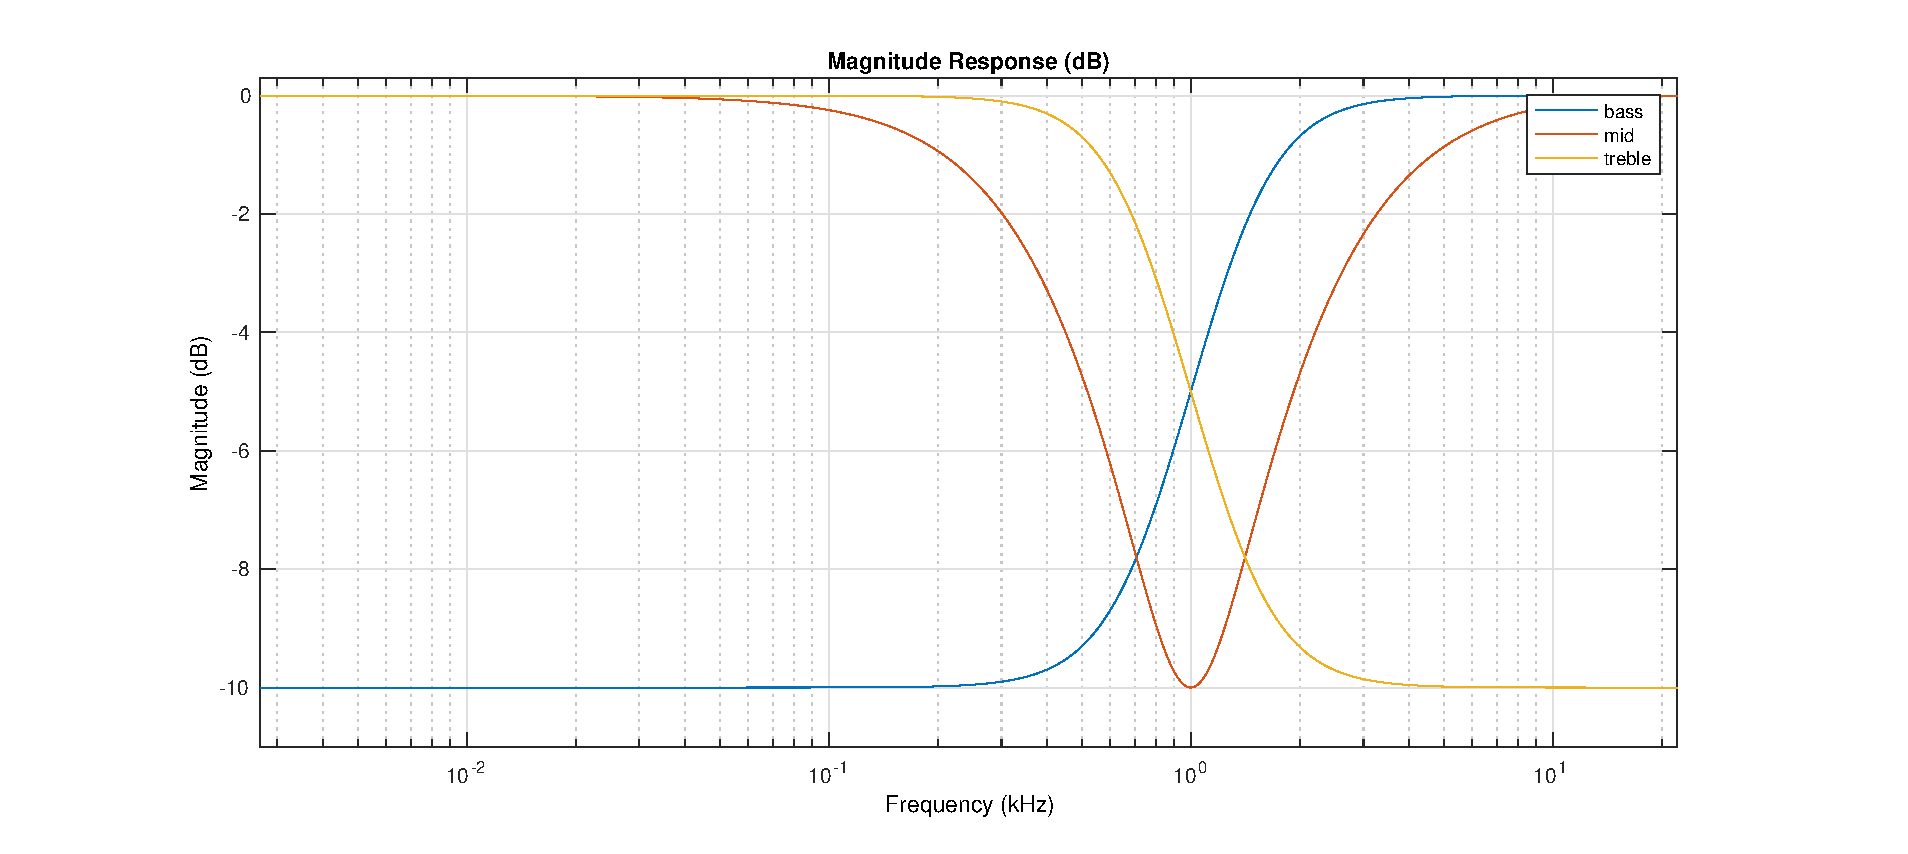
\includegraphics[scale=0.6]{./figs/eq-response.eps}        
    \caption{Magnitude Response of 3-Band EQ}
    \label{fig:eq-reponse}
\end{figure}
\end{centering}

\medskip
Control of the bass band is implemented using a low shelve biquad IIR filter; as the bass control is decreased, the gain moves becomes negative and attenuates the frequencies below 1kHz.
As before, the filter coefficients are calculated in the \lstinline{IIRFilter} constructor, using the following equations for a low shelf.

\begin{center}
    \begin{minipage}{.5\linewidth}
        \begin{equation*}
            \begin{aligned} 
                &a_0 = (A + 1) + (A - 1)cos(\omega_ 0) + 2\sqrt{A} \alpha \\
                &a_1 = -2((A - 1) + (A + 1)cos(\omega_ 0)) \\
                &a_2 = (A + 1) + (A - 1)cos(\omega_ 0) - 2\sqrt{A} \alpha
            \end{aligned}
        \end{equation*}
        \end{minipage}%
        \begin{minipage}{.5\linewidth}
        \begin{equation}
            \begin{aligned}
                &b_0 = A((A + 1) - (A - 1)cos(\omega _0) + 2\sqrt{A} \alpha) \\
                &b_1 = 2A((A - 1) - (A + 1)cos(\omega _0)) \\
                &b_2 = A((A + 1) - (A - 1)cos(\omega_ 0) - 2\sqrt{A} \alpha)
            \end{aligned}
        \end{equation}
    \end{minipage}
\end{center}

The treble band is implemented using a high shelve biquad IIR filter; as the treble control is decreased, the gain moves becomes negative and attenuates the frequencies above 1kHz.
Its filter coefficients are calculated using the same equations as the high shelf filter used previously for the woofer correction filter.

\medskip
Mid band control is achieved through a peaking filter, frequencies around 1kHz are attenuated as the mid control is reduced from 0dB to -15dB.
The coefficients are calculated using the following equations.

\begin{center}
    \begin{minipage}{.5\linewidth}
        \begin{equation*}
            \begin{aligned} 
                &a_0 = 1 + \frac{\alpha}{A} \\
                &a_1 = -2cos(\omega_ 0) \\
                &a_2 = 1 - \frac{\alpha}{A}
            \end{aligned}
        \end{equation*}
        \end{minipage}%
        \begin{minipage}{.5\linewidth}
        \begin{equation}
            \begin{aligned}
                &b_0 = 1 + \alpha A) \\
                &b_1 = 2 - cos(\omega _0) \\
                &b_2 =1 - \alpha A
            \end{aligned}
        \end{equation}
    \end{minipage}
\end{center}


% interleaving etc
\section{Hardware Interface and User I/O}
\subsection{Hardware Setup}
When the client is launched, some initial setup is required to enable audio output.
This is achieved through interfacing with the hardware using the $I^2C$ protocol and GPIO, the wiringPi library is used to do this.
This setup has previously been conducted using a separate bash script that would be executed on start-up, this is now being achieved in the main executable, the client.
Setup code is contained within the constructor of the \lstinline{HardwareController} class, a different version of this was written for the different sound cards.
A UML class diagram of the \lstinline{HardwareController} class can be seen in figure \ref{fig:hardware-uml}.

\begin{figure}[H]
    \centering
    \begin{tikzpicture}
        \umlclass{WifiHifi::HardwareController}{  
        - dbVols : int* \\
        - vol : int \\
        - downFlag : IIRCoeffs\textunderscore t* \\
        - timer : QPointer<<QTimer>> 
        }{
        HardwareController() \\
        \char`\~ HardwareController() \\
        \underline{+ VolumeUpISR() : void} \\ 
        \underline{+ VolumeDownISR() : void} \\ 
        \underline{+ PowerOffISR() : void} \\ 
        \underline{+ SetVolume() : void} \\
        \underline{+ GetVolume() : int} \\ 
        - PowerTimeout() : void 
        }
    \end{tikzpicture}
    \caption{HardwareController UML Class Diagram}
    \label{fig:hardware-uml}
\end{figure}

\medskip
The first generation card uses the PCM5102A DAC and MAX9744ETH amplifier, both of which require initial setup.
The PCM5102A's mute pin is driven low and the MAX9744ETH's enable pin is driven high to ensure that audio output is enabled.
The default volume for the MAX9744ETH is set at zero (linear) using $I^2C$.

\medskip
The second generation card utilises the TAS5805M integrated DAC and amplifier, its initial setup is significantly more complex than the PCM5102A and MAX9744ETH.
Its enable pin is first driven high using GPIO before additional configuration is set using $I^2C$ for a large number of values and registers.
To ease this process, the Texas Instruments Pure Path configuration tool was used to generated the required values to set.
These are represented as a large array of required values and registers in a header file, they are set by simply looping through the entire array and writing over $I^2C$.

\medskip
A very basic Pure Path configuration was used that includes no use of the hardware DSP filters, the only values that were experimented with were the volume level values.
A ceiling volume is set as -10dB by writing the volume registers for the right and left channel, software attenuation is used for the second sound-card so the hardware volume level is fixed. 
Replacing the software DSP with the internal filters of the device to alleviate processor load, and a full investigation into the device's capabilities, is a potential area of future work.

\subsection{Buttons and Switches}
Three buttons were included to provide basic volume and power-down functionality to the user. 
The volume buttons will trigger edge triggered interrupts on their GPIO input pins, the interrupt service routines (ISR) will either increase or decrease the volume by a set value until either the minimum or maximum linear value is reached.
For the first generation card, the maximum and minimum values are 60 and 0 respectively as these are the values accepted by the MAX9744ETH's volume register.
Conversely, since the second generation card uses software attenuation, these values are 0 and 1.

\medskip
A master power switch was included that entirely cuts the power to the RPI. 
To prevent potential corruption of the SD card when the power is immediately removed, a third button was added to power-down the RPI in software.
The ISR for this button's input starts a five second timer, when the timer expires, if the button is still depressed, the executable exits and the parent bash script calls \lstinline{sudo shutdown now} to power-down the RPI.


\pagebreak

\section{Synchronisation}
\subsection{Overview}
It was noticed during initial testing that audio would stutter for a prolonged period of time (approximately five seconds) before resuming normal playback.
This was found to be caused for two reasons.
Firstly, due to the JACK server being entirely decoupled from the ALSA output stream (processing thread), the sound-card was, in effect, running at a marginally different rate from the audio server.
Secondly, the \lstinline{SlaveProcessor::process()} callback would fail to be called by the server on some occasions, this would cause the entire audio stream to drop out for the cycles elapsed until the server would resume delivering audio.

\subsection{Drift Correction}
\medskip
The JACK server waits in the current process cycle until it receives a sync packet from the master JACK server on the user's PC, this ensures that each server is in sync for a given cycle.
From this, it can be concluded that by synchronising the output stream (the processing thread) of each speaker with its local server, each speaker is synchronised to the master server and thus, each other.

\medskip
Drift correction is performed in the processing thread before reading from the output buffer;
this involves determining how many samples the output stream is out of sync with the server and applying PI control to resize the output buffer, compensating for running either behind or ahead of the server.
A block diagram of the PI controller can be seen in figure \ref{fig:pi-controller}.

\begin{figure}[H]
    \centering
    \begin{signalflow}{}
        % - delay element
        \begin{scope}
            \node [input] (jack-written) {$N_{j}(n)$};
            \node [adder] (sum1) [right from=jack-written] {};
            \node [input] (alsa-written) [above from=sum1] {\nodepart{above}{$N_{a}(n)$}};
            \node [node] (node1) [right from=sum1] {};
            \node [node] (node0) [right from=node1, fill=white, draw=white] {};
            \node [delay] (integ) [below from=node0, fill=yellow!20] {$\int$}; 

            \node [delay] (Ki) [right from=integ, fill=yellow!20] {$K_{i}$}; 
            \node [multiplier] (neg1) [right from=Ki] {\nodepart{below}{-1}};

            \node [delay] (Kp) [right from=node0, fill=yellow!20] {$K_{p}$}; 
            \node [multiplier] (neg2) [right from=Kp] {\nodepart{above}{-1}};

            \node [adder] (sum2) [right from=neg2] {};
            \node [delay] (buffer-size) [right from=sum2, fill=yellow!20] {$M_{buff}$};
            \node [output] (out) [right from=buffer-size] {$N_{new}$};
            \node [input] (setpoint) [above from=sum2] {\nodepart{above}{$1$}};

            \path[r>] (jack-written)  -- (sum1);
            \path[r>] (alsa-written)  -- (sum1);
            \path[r] (sum1)  -- (node1);
            \path[r>] (node1)  -- (Kp);
            \path[r>] (Kp)  -- (neg2);
            \path[r>] (neg2)  -- (sum2);
            \path[r>] (sum2)  -- (buffer-size);
            \path[r>] (buffer-size)  -- (out);

            \path[r>] (node1)  |- (integ);
            \path[r>] (integ)  -- (Ki);
            \path[r>] (Ki)  -- (neg1);
            \path[r>] (neg1)  -| (sum2);
            \path[r>] (setpoint)  -- (sum2);

        \end{scope}
    \end{signalflow}
    \caption{Drift Correction PI Controller}
    \label{fig:pi-controller}
\end{figure}

In the situation that the output stream is very out of sync with the server, then the drift correction will force the the stream into sync using the \lstinline{AlsaController}.
The tolerance in which the stream may jitter is set at 256 samples for either rushing ahead, or lagging behind.
If the output stream is detected to have rushed ahead of the server by the tolerance, the playback is rewound.
If the output stream is detected to have lagged behind of the server by the tolerance, a temporary buffer of 256 samples is immediately written to force the stream to ``catch up'' with the server. 
This can be seen in the following listing, note that an FIR filter is reset, this is because the raw offset is smoothed. 

\begin{lstlisting}[language=c++, caption={Hard Rewind or Buffer Padding for Unsynchronised Streams}]
    if (offset < rushTolerance)
    {
        /* ALSA is running ahead so force a rewind */
        m_dac->Rewind(-1*deltaK);
        m_driftFilter->reset();
        m_integDeltaK = - (m_resampleMean - 1.0) * (1 / K) * (1 / Ki);
        std::cout << "ALSA IS RUSHING" << std::endl;
    }
    if (offset > dragTolerance)
    {
        /* ALSA is lagging behind so pad a temporary buffer and write */
        while (offset > 0) 
        {
	        to_write = (offset > 512) ? 512 : offset;
            m_dac->WriteInterleaved(m_padBuffer, static_cast<int>(to_write));
	        offset -= to_write;  
	    }
        m_driftFilter->reset();
        m_integDeltaK = - (m_resampleMean - 1.0) * (1 / K) * (1 / Ki);  
    }
\end{lstlisting}
It is generally more favourable for the output stream to lag a little behind the server rather than rushing ahead, this is because a rewind is much more noticeable than padding a buffer for 256 samples.
It was found that the controller would work reasonably well with the offset very gradually reaching the dragging tolerance, when the stream was forced back into sync through padding, it was not noticeable to the human ear.
The proportional gain, $K_p$ was set at $\frac{1}{100000}$ and the integral gain, $K_i$, set at $\frac{1}{10000}$.
The integral term was set as the dominant term as the controller was found to work best acting mostly on the accumulated error, this is because the output streams falls out of sync slowly.

\subsection{Missed Process Callbacks}

\begin{figure}[H]
\begin{tikzpicture}
    \begin{axis}[
        width=\textwidth, 
        height=\axisdefaultheight, 
        xtick={0,0.1,...,1},
        xmin=0,
        xmax=1,
        ytick ={0, 1},
        ymax = 1.5,
        restrict x to domain*=0:1,
        restrict y to domain*=0:1,]
    %\addplot table [mark=none, x=t, y=a, col sep=comma] {./data/saleae-outputs/sync.csv};
    
    \addplot table [mark=none, x=t, y=b, col sep=comma] {./data/saleae-outputs/run2.csv};
    \end{axis}
\end{tikzpicture}
\end{figure}

\section{Desktop Application}
\subsection{Overview}
The desktop application, WifiHifi Controller, allows the user to vary the tone controls and volume levels remotely over the local network.
It was written using the C++ Qt framework, a library for multitasking and GUI applications.
A screenshot of the main window can be seen in figure \ref{fig:app-screenshot}.

\begin{figure}[H]
    \centering
    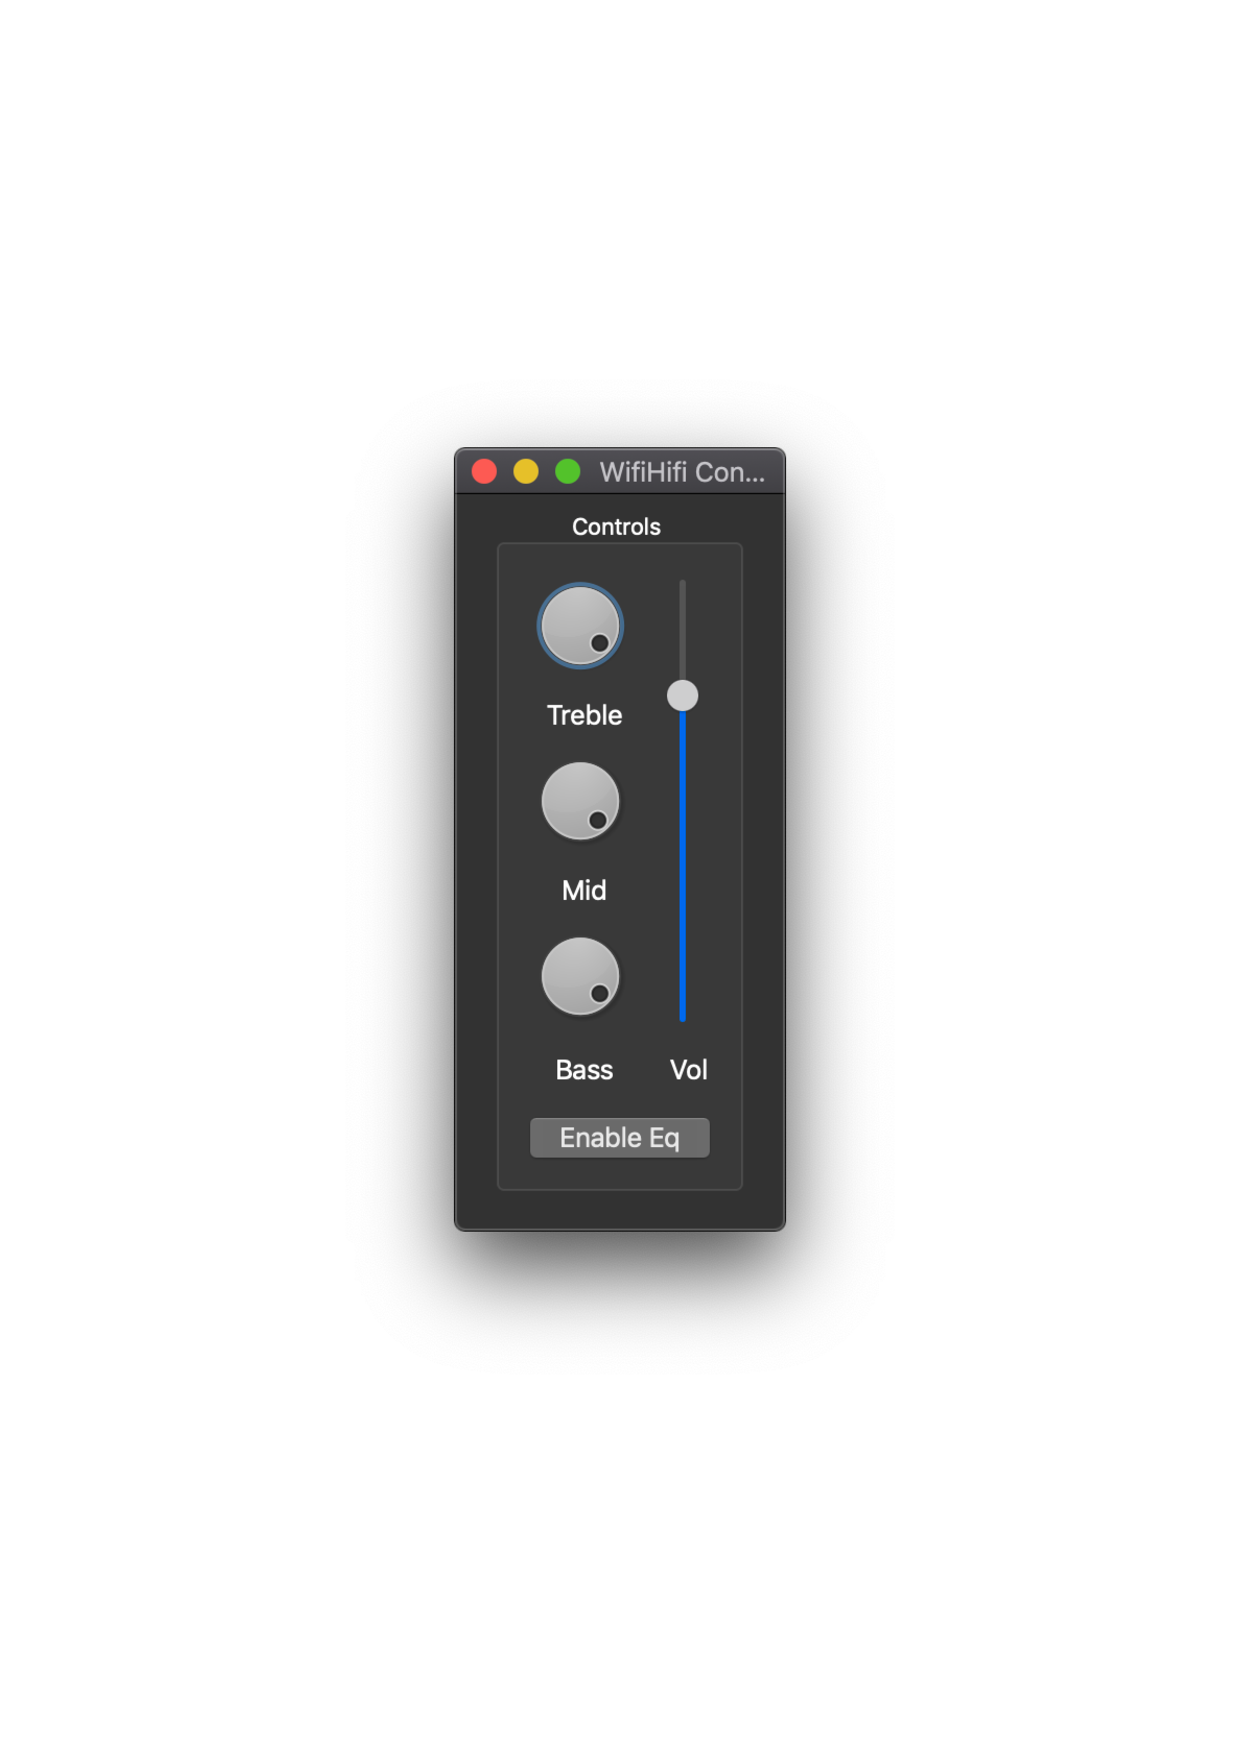
\includegraphics[scale=0.6]{./figs/app-screenshot.pdf}        
    \caption{Screenshot of WifiHifi Controller Main Window}
    \label{fig:app-screenshot}
\end{figure}

\subsection{Controls}
EQ values for each band and volume requests are sent using UDP, they are sent to a single multicast IP address, 239.1.1.1, on port 1234.
This ensures that all speakers receive the values without requiring to unicast indivdual values to each speaker which would take up more bandwidth.
When a control is moved by the user, the new value is appended to an outgoing datagram and sent to the multicast address.
The datagram is prepended with a letter indicated what control the value corresponds to: ``B'' for bass, ``M'' for mid etc.
Each speaker parses these datagrams and performs the adjustments required.




\end{document}